\chapter{Durchführung}
\label{sec:durchfuerung}

Im ersten Versuchsteil werden die drei Proben mittels Sinnesprüfung untersucht. Alle Proben werden hierfür durchgeschüttelt, um homogenisierte Wasserproben zu erhalten und anschließend in Klarglasgefäße, in diesem Fall drei Erlenmeyerkolben, umgefüllt. Vor einem weißen Hintergrund platziert (siehe Abb. \ref{fig:proben}), erfolgt nun die optische Sinnesprüfung mit Einschätzung von Färbung und Trübung nach den Einstufungen in Tab. \ref{tab:einstufungen}. 

\vspace*{-2.5mm}
\renewcommand{\arraystretch}{1.2}
\begin{table}[h!]
	\centering
	\caption{Einstufungen der Färbung und Trübung nach Praktikumsskript \cite{Skript}}
	\label{tab:einstufungen}
	%\resizebox{10cm}{!}{
	\begin{tabulary}{\textwidth}{C|CCCC}
		\hline
		\textbf{} & \textbf{Stufe 1} & \textbf{Stufe 2} & \textbf{Stufe 3}& \textbf{Stufe 4} \\ 
		\hline
		\textbf{Färbung} & farblos & schwach & stark gefärbt& -\\
		\textbf{Trübung} & klar & schwach getrübt & stark getrübt & undurchsichtig\\
		\hline
	\end{tabulary}
	%}
\end{table}
\FloatBarrier

%Tabelle Ende


%Start
\begin{figure}[h!]
	\centering
	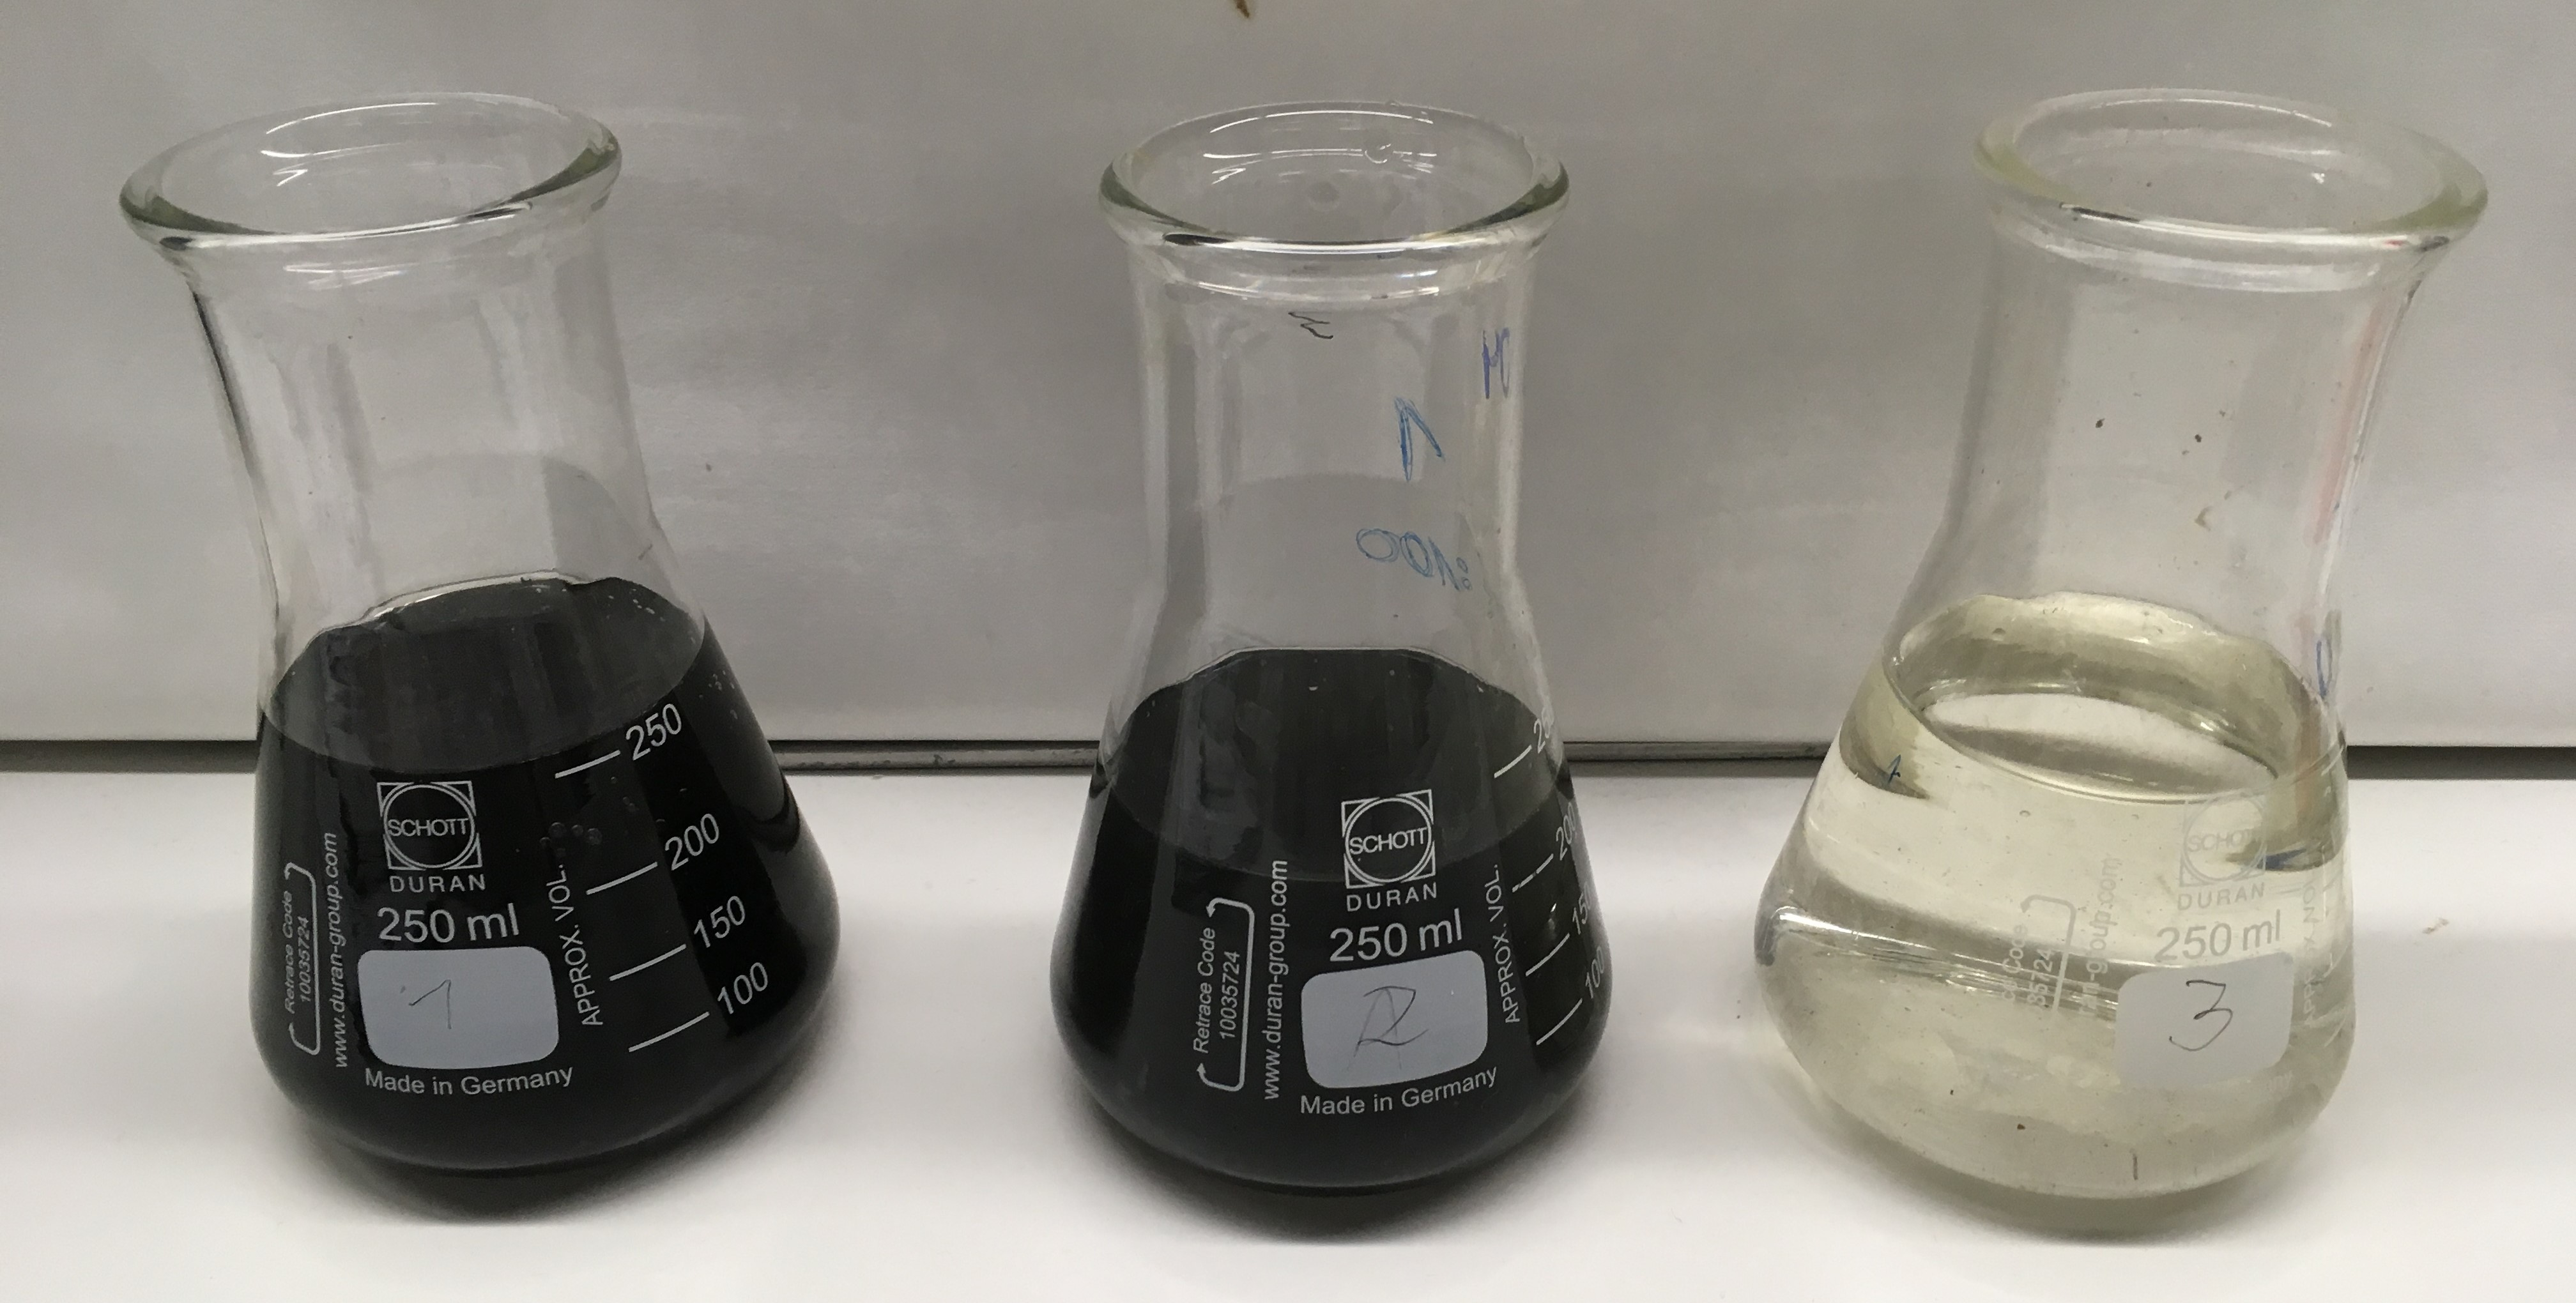
\includegraphics[width=0.45\textwidth]{img/proben}
	\caption{Foto der Abwasserproben 1 bis 3}
	\label{fig:proben}
\end{figure}
\FloatBarrier
%Ende
%Tabelle START


Des Weiteren werden sind die Proben olfaktorisch in Bezug auf Intensität und Art mit den Einstufungen aus Tabelle \ref{tab:einstufung_geruch} zu kategorisieren und mit charakteristisch-chemischen Gerüchen zu vergleichen.

\vspace*{-2.5mm}
\renewcommand{\arraystretch}{1.2}
\begin{table}[h!]
	\centering
	\caption{Wahrgenommene Einstufungen der Färbung und Trübung der Abwasserproben 1 bis 3}
	\label{tab:einstufung_geruch}
	%\resizebox{10cm}{!}{
	\begin{tabulary}{\textwidth}{C|L}
		\hline
		\textbf{} & \textbf{Beschreibung} \\
		\hline
		\textbf{Intensität}	& ohne - schwach - stark\\
		\textbf{Art}		& erdig, torfig, muffig, fischig, jauchig, modrig, chemisch\\
		\textbf{charak.-chemisch  }	& \ce{H2S}, Chlor, Mineralöl, Benzin, Teer, Phenol\\
		\hline
	\end{tabulary}
	%}
\end{table}
\FloatBarrier
\vspace*{-2.5mm}

%Tabelle Ende

\newpage

Im zweiten Versuchsteil werden die Proben elektrochemisch mittels pH-Wert-Elektrode und 2-in-1 Potentiometer-Temperatursensor analysiert. Die pH-Wert-Elektrode ist dabei auf \SI{25}{\celsius} kalibriert und untersucht werden die drei Abwasserproben einmal mit und einmal ohne vorangegangene Vakuumfiltration (siehe Abb. \ref{fig:proben_filter}). \linebreak Während der elektrochemischen Messungen wird die jeweils zu untersuchende Probe mittels Magnetrührer bei ca. \SI{300}{\rpm} homogen gehalten.

%Start
\begin{figure}[h!]
	\centering
	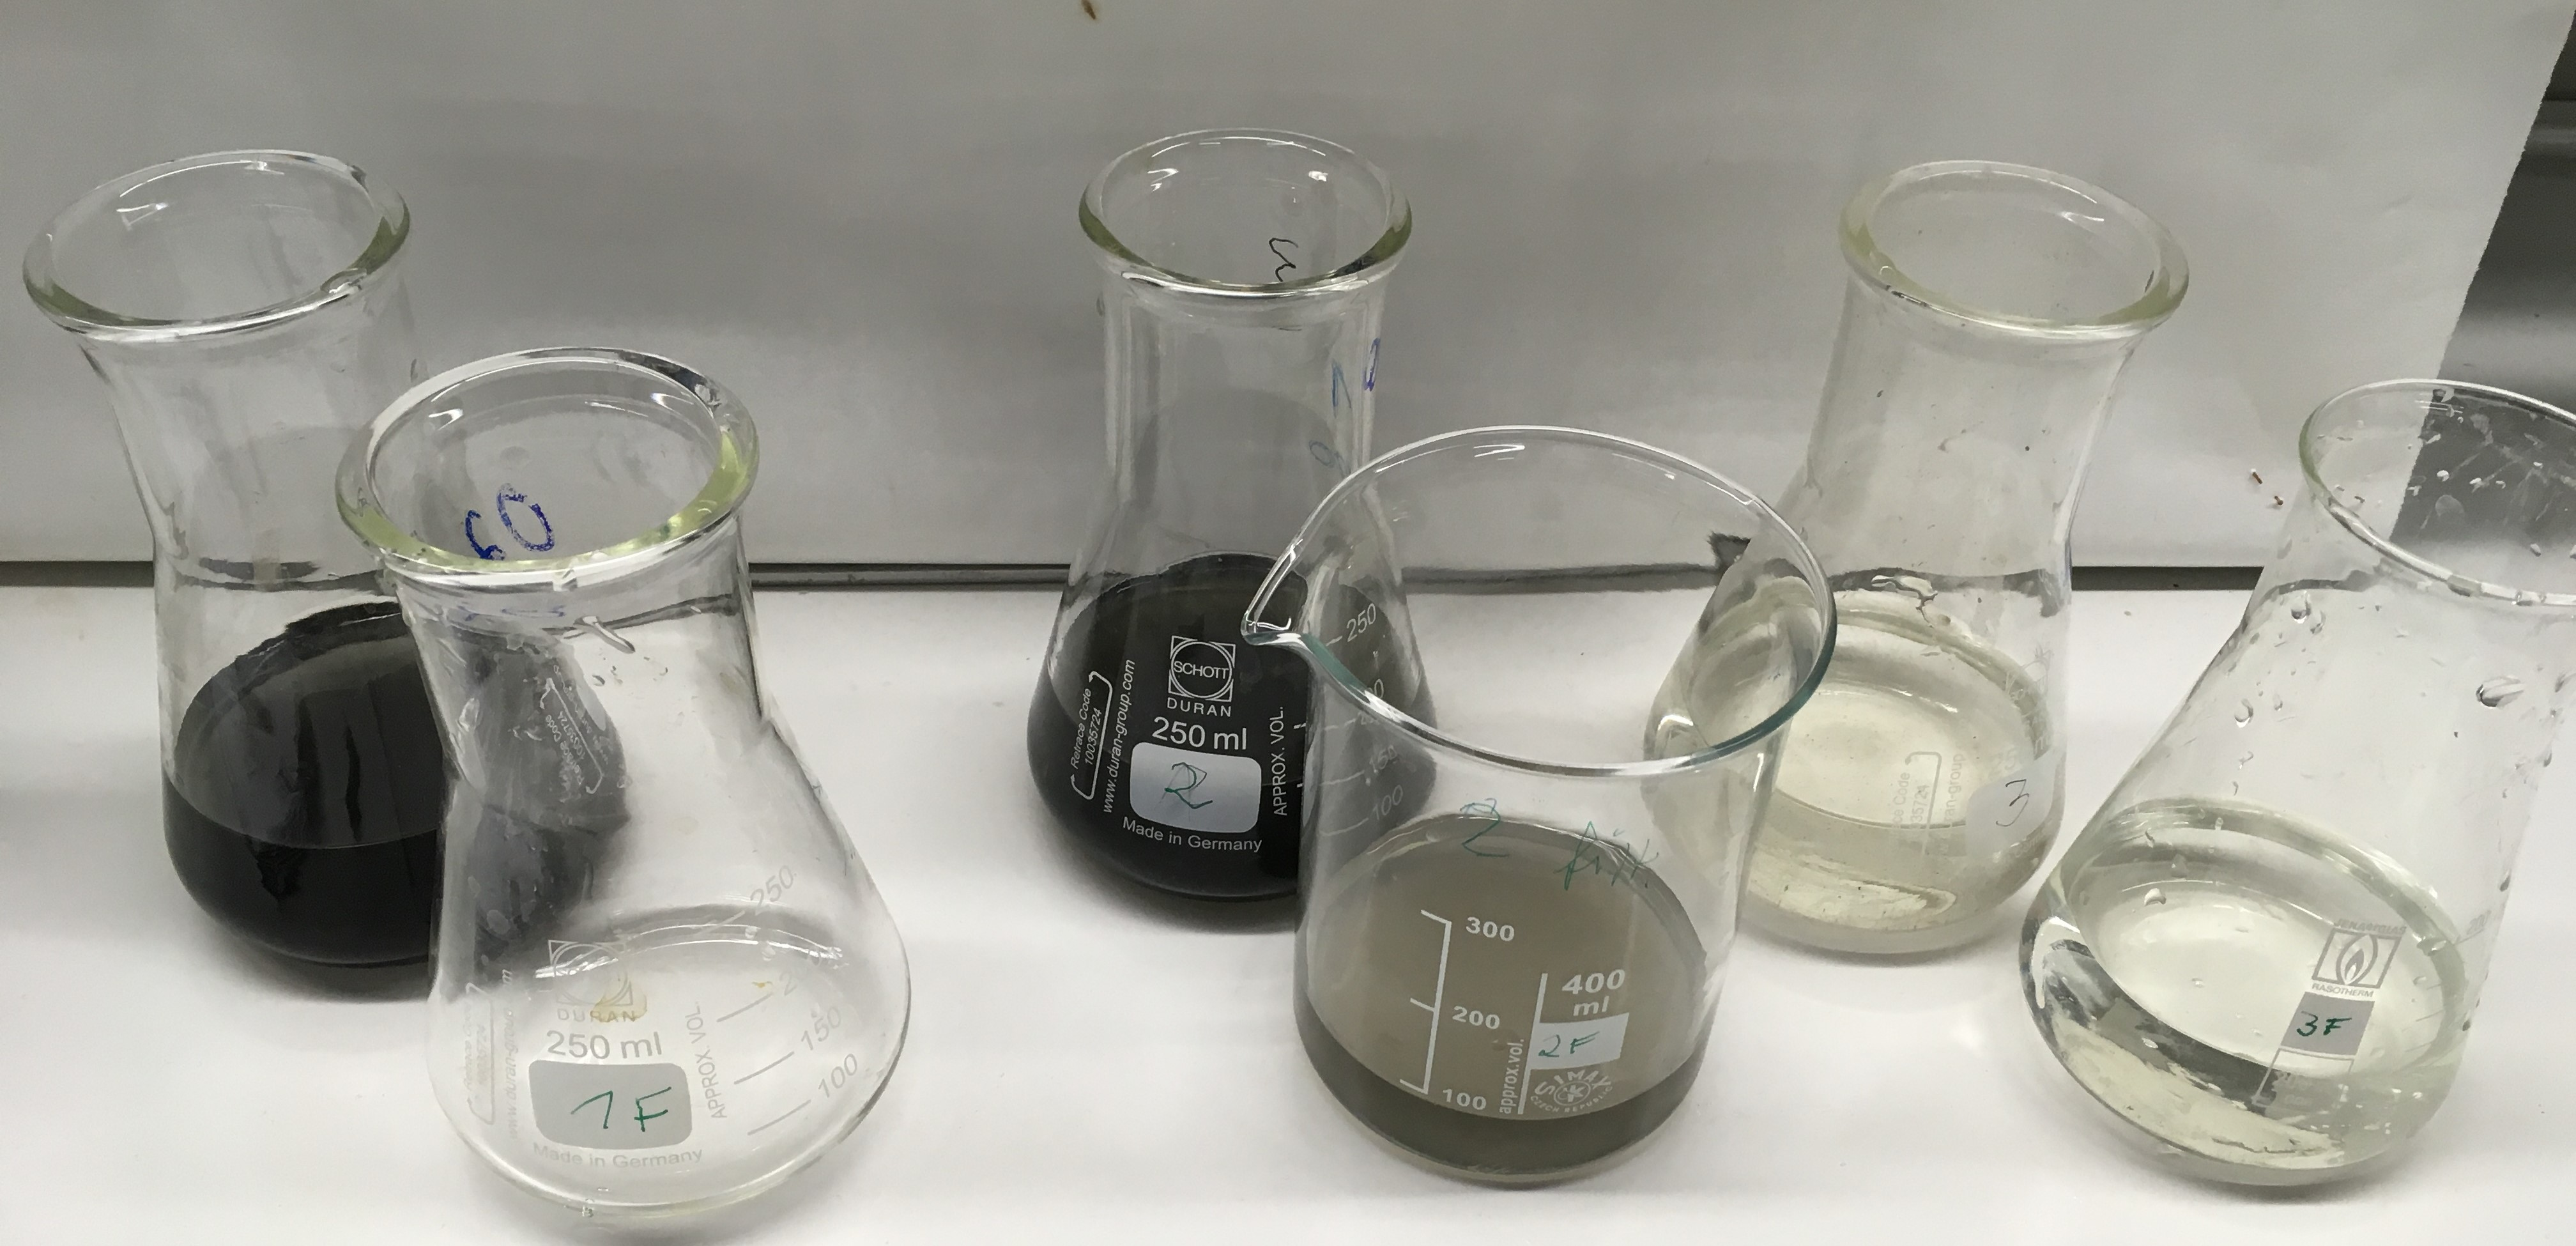
\includegraphics[width=0.45\textwidth]{img/proben_filter}
	\caption{Foto der Abwasserproben 1 bis 3 (filtriert und unfiltriert)}
	\label{fig:proben_filter}
\end{figure}
\FloatBarrier
%Ende

Im dritten und letzten Versuchsabschnitt werden die zuvor gefilterten Proben auf ihre enthaltenen Ionen geprüft. Dafür werden die Proben wiedermals durch schütteln homogenisiert und dann im ersten Zug via Schnellteststreifen analysiert. Es werden Schnellteststreifen der Firma \textsc{Chemsolute$^{\textsuperscript{\textregistered}}$} genutzt, welche die Proben auf Nitrit-, Nitrat- und Phosphat-Ionen testen und mittels abgestufter Farbskala eine grobe Beurteilung über den Gehalt der Ionen in $\left[\si{\milli \gram}\right]$ ermöglichen. Beispielhaft sind in Abbildung \ref{fig:phosphat_test} die Schnelltestpackungen mit den Farbskalen und danebenliegenden Phosphat-Teststreifen zu sehen.\\
Im zweiten Zuge des Versuchsabschnittes werden die Proben mittels Reflektometer geprüft. Dafür wird das Messgerät mit dem der Packung beiliegenden Barcode kalibriert und im Anschluss die Messsequenz per Knopfdruck gestartet. Auch hier werden wieder beigefügte Teststreifen verwendet und mit der Probe befeuchtet. Die Verweildauer in der Lösung ist dabei entweder der Packungsbeilage oder dem Messgerät zu entnehmen. In den letzten 5 Sekunden des Timers auf dem Reflektometer wird man aufgefordert den mit der Probe befeuchteten Teststreifen in den Stäbchenadapter einzuspannen und erhält binnen Sekunden den Messwert für das jeweilige Ion.
%Start
\begin{figure}[h!]
	\centering
	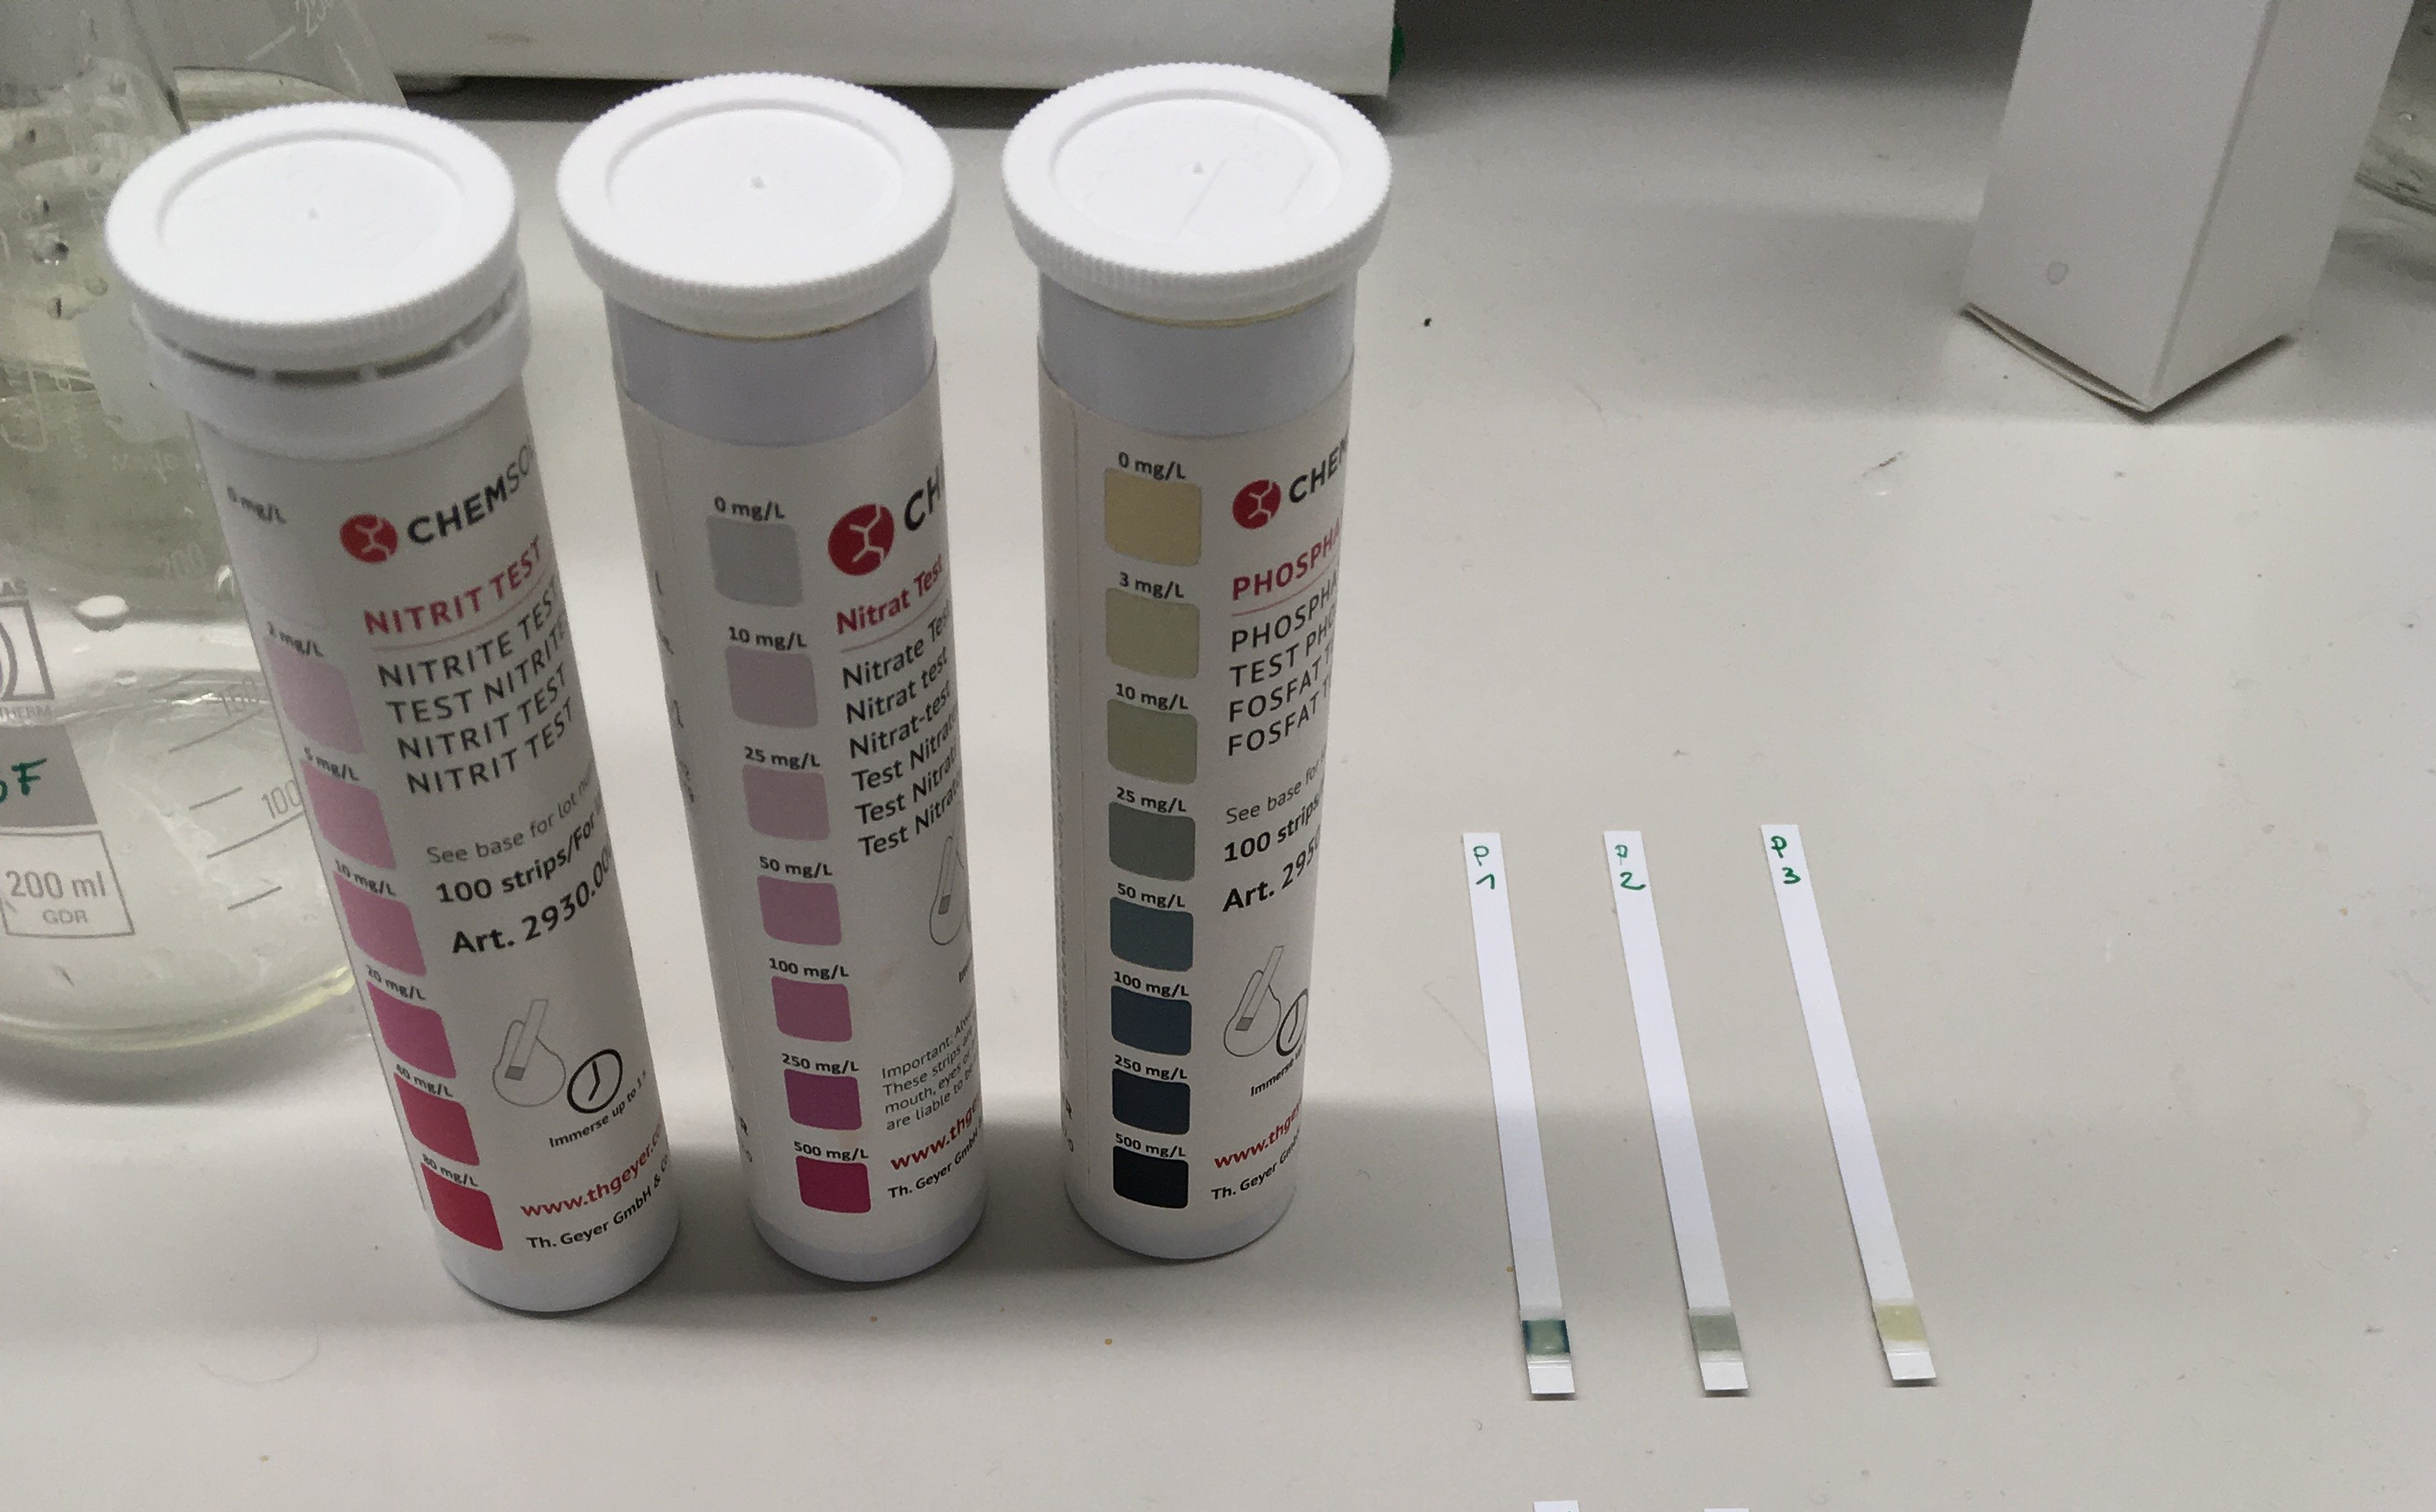
\includegraphics[width=0.45\textwidth]{img/phosphat}
	\caption{Foto der Schnelltestpackungen mit jeweiliger Farbskala und danebenliegenden Phosphat-Teststreifen}
	\label{fig:phosphat_test}
\end{figure}
\FloatBarrier
%Ende